\section{Exemplo de operação}
\label{sec:exemplo}

Esta seção mostra o exemplo do funcionamento 

O experimento apresentado é baseado na geração simulada de trilhas de estudantes dentro de um contexto de Educação Ubíqua. Educação Ubíqua pode ser compreendida como processos educacionais que ocorrem em qualquer lugar, a qualquer tempo e com qualquer dispositivo, de forma contínua, contextualizada e integrada ao cotidiano do aprendiz \cite{barbosa05}.

O cenário simula um curso de programação em linguagens orientadas a objeto. O curso consiste em um conjunto de módulos relacionados a orientação a objetos que o usuário transfere para seu dispositivo móvel e estuda através dele. Destes módulos fazem parte conceitos básicos da matéria (classes, herança, {\em interfaces} e ponteiros) e linguagens de programação orientadas a objeto (C++, Python e Java). O estudante não é obrigado a concluir todos os módulos. No final do curso, no entanto, ele deve escolher a linguagem de programação que ele utilizará para responder as questões da prova final. Dependendo da linguagem que escolher, ele deve ter concluído, no mínimo, os módulos referentes àquela linguagem.

As dependências dos módulos estão representadas na Figura~\ref{fig:cen1_modulos}. Por exemplo, caso o aluno decida realizar a prova em Java, ele deve ter estudado classes, herança e {\em interfaces}, além do Java propriamente dito. Como a linguagem Java não contém o conceito de ponteiros, ele não é obrigado a ter cursado este módulo.

\begin{figure}
  \begin{center}
    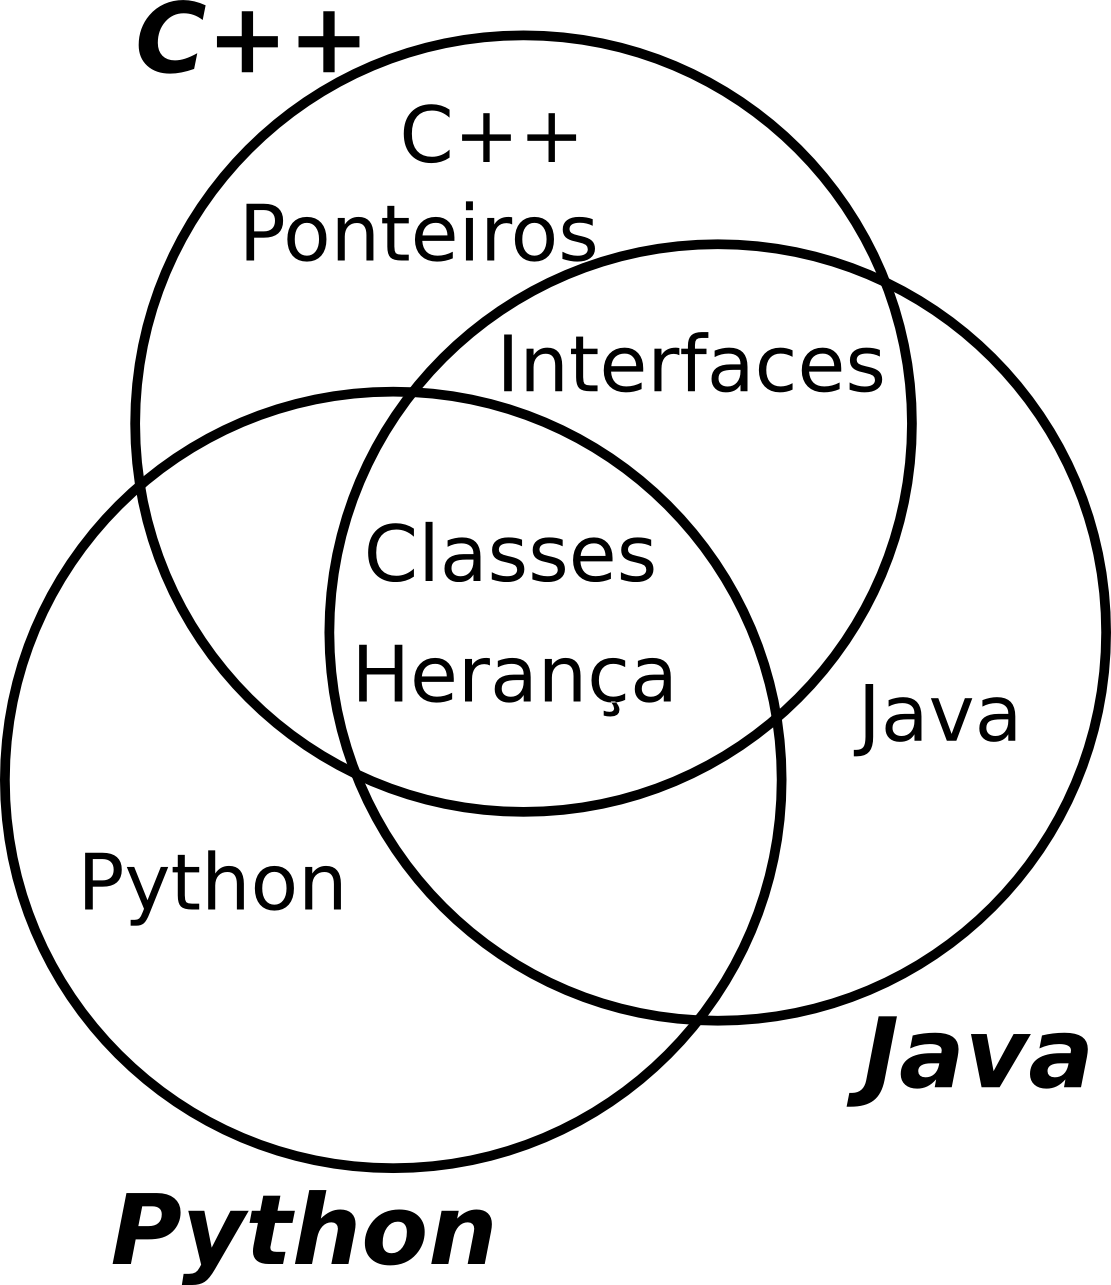
\includegraphics[width=0.15\textwidth]{imagens/cen1_modulos.png}
  \end{center}
  \caption{\textbf{Módulos de estudo obrigatórios}}
  \label{fig:cen1_modulos}
\end{figure}

Neste experimento, aplicativo de educação ubíqua distribui os objetos de aprendizagem de forma contextualizada. O aplicativo registra em um gerenciador de trilhas cada vez que um módulo é iniciado ou concluído. Tanto o aplicativo quanto o gerenciador de trilhas são simulados.

% TODO - figura para vinculação 

Cada evento (início ou conclusão de um objeto de aprendizagem) é registrado contendo as seguintes informações: (i) entidade que realizou o evento, (ii) objeto de aprendizagem, (iii) tipo de evento (início ou conclusão), (iii) data e hora e (iv) se é a primeira vez que o estudante realiza este tipo de evento. No cenário simulado, os eventos descritos na Tabela~\ref{tab:eventos} foram registrados pelo aplicativo no gerenciador de trilhas durante um período de um dia.

\begin{table}\centering\footnotesize
  \begin{tabular*}{0.47\textwidth}{@{}lllll@{}}
    \toprule
    Entidade & Objeto de    & Tipo de & Data e Hora & Primeira \\
             & aprendizagem & evento  &             & vez? \\
    \midrule
    Andre    & Interfaces   & Início  & 09/07/2012 08:12 & Sim \\
    Andre    & Classes      & Término & 09/07/2012 09:28 & Sim \\
    Maria    & Herança      & Término & 09/07/2012 09:32 & Sim \\
    Andre    & Java         & Término & 09/07/2012 11:14 & Sim \\
    Maria    & Interfaces   & Término & 09/07/2012 11:28 & Sim \\
    Andre    & Ponteiros    & Início  & 09/07/2012 13:58 & Sim \\
    Andre    & Ponteiros    & Término & 09/07/2012 14:12 & Sim \\
    Andre    & Java         & Término & 09/07/2012 16:18 & Não \\
    \bottomrule
  \end{tabular*}
  \caption{\textbf{Trilha gerada pelo aplicativo}}
  \label{tab:eventos}
\end{table}

No cenário apresentado, deseja-se atualizar o perfil de uma entidade, inserindo a informação de proficiência dela em determinada disciplina. Esta informação será utilizada posteriormente pela aplicação para determinar se o estudante está apto a realizar o teste. Para que o eProfile possa ser capaz de inferir esta informação, a aplicação precisa, ao montar as trilhas, enviar informações suficientes para que o eProfile possa montar a ontologia que represente a situação atual. Neste experimento, um exemplo de informação deste tipo são as dependências entre as disciplinas. A Figura~\ref{fig:cen1_ontologia} mostra a ontologia montada pelo eProfile baseado nas trilhas enviadas da aplicação o gerenciador de trilhas, e do gerenciador ao eProfile.

\begin{figure}
  \begin{center}
    
\includegraphics[width=0.5\textwidth]{cen_ontologia.png}
  \end{center}
  \caption{\textbf{Ontologia do cenário apresentado}}
  \label{fig:cen1_ontologia}
\end{figure}

Além das trilhas, a aplicação deve enviar as regras de inferência ao eProfile. Estas regras serão utilizadas pelo eProfile para inferir as trilhas e gerar o perfil. Neste experimento, para que o eProfile possa identificar se uma entidade é proficiente em alguma disciplina, são necessárias três regras: (i) a identificação dos objetos de aprendizagem requeridos para a proficiência na disciplina; (ii) a identificação dos objetos de aprendizagem concluídos pelo estudante e; (iii) a verificação se os objetos requeridos foram concluídos.

A primeira regra está apresentada na Figura~\ref{cod:regra1}, sendo composta por uma classe escrita em OWL\footnote{Embora o eProfile utilize internamente a sintaxe OWL/RDF \cite{owl-guide}, a sintaxe Manchester-OWL está sendo usada neste artigo por ser mais compacta e amigável \cite{owl-manchester}.}. Para que um estudante seja considerado proficiente em Java, ele deve ter concluído os objetos de aprendizagens que fazem relação com a linguagem Java (neste caso classes, herança e {\em interfaces}, na linha 4), bem como o objeto de aprendizagem da própria linguagem Java (linha 3). 

\begin{figure}
\begin{lstlisting}
Class: <el:JavaRequirement>
    EquivalentTo: 
        <el:Java>
         or (<el:relatesTo> some <el:Java>)
\end{lstlisting}
\caption{\textbf{Regra de requerimentos para disciplina}}
\label{cod:regra1}
\end{figure}

O segundo passo é a identificação dos objetos de aprendizagem concluídos pelo estudante relacionados ao Java. Esta regra é apresentada na Figura~\ref{cod:regra2}. Assim, são considerados apenas os eventos de conclusão de objeto de aprendizagem (linha 3) realizados pela entidade (linha 4), relacionados ao Java (linha 5) e que tenham sido realizados pela primeira vez (linha 7), uma vez que o aluno pode estudar o mesmo material várias vezes. O parâmetro \texttt{[?entity]} será substituído pela entidade na execução da regra de cada perfil. É importante notar que para verificar se a disciplina está relacionada ao Java, a regra criada na Figura~\ref{cod:regra1} é utilizada (linhas 5 e 6).

\begin{figure}
\begin{lstlisting}
Class: <el:JavaLessonsTaken>
    EquivalentTo: 
        <el:FinishedLOEvent>
	 and (<el:hasEntity> some [?entity])
         and (<el:hasLearningObject> some 
	                    <el:JavaRequirement>)
         and (<el:isFirstTime> value true)
\end{lstlisting}
\caption{\textbf{Regra de objetos de aprendizagem concluídos}}
\label{cod:regra2}
\end{figure}

Uma vez que estas duas regras estejam criadas na ontologia, o eProfile executa o raciocinador, que gera uma nova ontologia OWL, com as classes inferidas identificadas como filhas das classes criadas.

A terceira regra é uma regra de atualização de perfil (Figura~\ref{cod:regra3}. Nesta regra, são comparados o número de módulos Java (regra da Figura~\ref{cod:regra1}) com o número de objetos de aprendizagem relacionados ao Java que foram concluídos pela entidade (regra da Figura~\ref{cod:regra2}). Se o número for igual, o usuário é considerado proficiente, e esta regra é atualizada no perfil da entidade.

\begin{figure}
\begin{lstlisting}
JavaProficience <= 
  (Count(SubClasses(JavaRequirement))) equals
          (Count(SubClasses(JavaLessonsTaken)))
\end{lstlisting}
\caption{\textbf{Regra de proficiência}}
\label{cod:regra3}
\end{figure}

No experimento realizado, verificou-se que nenhum dos usuários foi considerado proficiente em Java. Isto ocorre pois, de acordo com a Tabela~\ref{tab:eventos}, nenhum dos usuários chegou a concluir todos os módulos requeridos para a proficiência nesta linguagem. Assim, o perfil destas entidades foi atualizado como ``Não-proficiente em Java''. Como esta regra será executada periodicamente, uma vez que os usuários tenham concluído todos os módulos requeridos, o perfil será atualizado como ``Proficiente em Java''.

